%!TEX root = ..\..\main.tex
\chapter{The Coupling Time on the Cycle}
\label{Ch:1D}

\lhead{Chapter \ref{Ch:1D}. \emph{The Coupling Time on the Cycle}}

	In this chapter we consider the Ising heat-bath Glauber dynamics (as described in Section \ref{sec:heat-bath glauber dynamics definition}) on the cycle $G_n = (\mathbb{Z}/n\mathbb{Z})$. The object of interest is the coupling time, $T_n$, which was defined in Section \ref{sec:the coupling time} but whose definition will be modified slightly in Section \ref{sec:information percolation on the cycle} to allow for simpler analysis. The main result establishes that $T_n$ converges in distribution to a Gumbel distribution at all temperatures. This confirms, for $d = 1$, a conjecture by \citeauthor{Collevecchio2017-nq} that the coupling time of the Ising heat-bath process on the lattice $G_L = (\mathbb{Z}/L\mathbb{Z})^d$ converges to a Gumbel distribution as $L \rightarrow \infty$ for all $\beta < \beta_C$ \cite[Conjecture 7.1]{Collevecchio2017-nq} (We treat higher dimensions, and more generally any vertex transitive graphs, in Chapter \ref{Ch:GeneralResults}). Of course, in one dimension, all temperatures are part of the high temperature regime [CITE], and likewise our result holds for any inverse-temperature $\beta$.

	\begin{theorem}
	\label{thm:Coupling Distribution on Cycle}
		Let $T_n$ be the coupling time for the continuous-time Ising heat-bath Glauber dynamics for the zero-field ferromagnetic Ising model on the cycle $(\mathbb{Z} / n\mathbb{Z})$. Then for any inverse-temperature $\beta$,
		\begin{equation}
			\lim_{n \rightarrow \infty} \prob\left[T_n < \frac{z + \ln n}{\theta}\right] = \euler^{-C_\theta \euler^{-z}}
		\end{equation}
		where $\theta = 1 - \tanh(2\beta)$ and $C_\theta$ is a positive constant bounded by
		\begin{equation}
			\frac{1}{2\sqrt{\frac{4}{\theta} - 1} - 1} \leq \lambda \leq 1.
		\end{equation}
	\end{theorem}

	The proof of Theorem \ref{thm:Coupling Distribution on Cycle} will be given in Section \ref{sec:proof thm coupling cycle} after the essential preliminaries are presented.

	\section{A new coupling on the cycle}
	\label{sec:information percolation on the cycle}
	% On the cycle, the heat-bath dynamics allow for a new set of updates rules, to replace those from \eqref{eq:plusorminusrules}. The changed update rules provide another construction for the coupling of $\mathscr{T}_t$ and $\mathscr{B}_t$ but preserve the distribution of the coupling time, $T_n$. We use these new update rules because they result in much simpler update histories.

	On the cycle, we will use a different coupling of $\mathscr{T}_t$ and $\mathscr{B}_t$ via a new set of update rules that will replace those from \eqref{eq:plusorminusrules}. The new update rules simplify our update histories greatly by ensuring that each of the update histories never contain more than one vertex at any one time. However, we must be cautious. The coupling time is not just a property of the heat-bath dynamics, but also of the specific coupling we chose. Hence, we will have to verify that switching to our new rules does not change the distribution of $T_n$. 

	The new update rules are defined by using almost the same construction as in Section \ref{sec:the coupling time}. The one difference is that we replace \eqref{eq:plusorminusrules} as follows. When vertex $i$ updates, instead of comparing $U$ to the probability $p_i(\sigma)$ to determine the new spin, we instead chose a new spin $\sigma_i'$ via
	% state that when vertex $i$ updates, a spin $\sigma_i'$ is chosen via
	\begin{equation}
	\label{eq:new update rules}
		\sigma_i' = \begin{cases}
			+1 & U < \theta/2,\\
			\sigma_{i-1} & \theta/2 \leq U < 1/2,\\
			\sigma_{i+1} & 1/2 \leq U < 1 - \theta/2,\\
			-1 & U \geq 1 - \theta/2.
		\end{cases}
	\end{equation}
	where $U \in [0,1]$ is an independent uniform random variable as before. It is easy to see that these update rules give rise to the same transition rates as those in \eqref{eq:plusorminusrules}. To show that the coupling time is unchanged, it is sufficient to verify that the joint jump probabilities of $(\mathscr{T}_t[i], \mathscr{B}_t[i])$ are unchanged for each possible configuration of spins of vertices $i-1$ and $i+1$. There are only nine possible configurations for the two neighbours of $i$ in the top and bottom chain since $\mathscr{B}_t[i] \leq \mathscr{T}_t[i], \forall t$. Likewise, there are only three possible configurations for the updated spins $(\mathscr{T}_t[i]', \mathscr{B}_t[i]')$. Hence, given vertex $i$ updates at time $t$, we can easily calculate all the required jump probabilities as shown in Table \ref{tab: joint jump probs}. These are unchanged whether using \eqref{eq:plusorminusrules} or \eqref{eq:new update rules} and so the new rules do not change the coupled dynamics.

	\begin{table}
	\begin{tabular}{c || c c c}
	\diagbox[]{		
		\begin{tabular}{@{}c@{}}
		$\mathscr{T}_t = \cdot$ \\ 
		$\mathscr{B}_t = \cdot$ 
		\end{tabular}
	}{
		$\prob[(\mathscr{T}_t[i]', \mathscr{B}_t[i]') = \cdot \,]$
	}
	&(1,1)&(1,-1)&(-1,-1)\\
	\hline
	\hline
		\begin{tabular}{@{}c@{}}
		$(\dots, 1, \sigma_i, 1,\dots)$ \\ 
		$(\dots, 1, \sigma_i, 1,\dots)$ 
		\end{tabular}
	&$1 - \theta$& 0 & $\frac{\theta}{2}$\\
	\hline
		\begin{tabular}{@{}c@{}}
		$(\dots, 1, \sigma_i, 1,\dots)$ \\ 
		$(\dots, 1, \sigma_i, -1,\dots)$ 
		\end{tabular}
	&$\frac{1}{2}$& $\frac{1-\theta}{2}$ & $\frac{\theta}{2}$\\
	\hline
		\begin{tabular}{@{}c@{}}
		$(\dots, 1, \sigma_i, 1,\dots)$ \\ 
		$(\dots, -1, \sigma_i, 1,\dots)$ 
		\end{tabular}
	&$\frac{1}{2}$& $\frac{1-\theta}{2}$ & $\frac{\theta}{2}$\\
	\hline
		\begin{tabular}{@{}c@{}}
		$(\dots, 1, \sigma_i, 1,\dots)$ \\ 
		$(\dots, -1, \sigma_i, -1,\dots)$ 
		\end{tabular}
	& $\frac{\theta}{2}$ & $1 - \theta$ & $\frac{\theta}{2}$ \\
	\hline
		\begin{tabular}{@{}c@{}}
		$(\dots, 1, \sigma_i, -1,\dots)$ \\ 
		$(\dots, 1, \sigma_i, -1,\dots)$ 
		\end{tabular}
	& $\frac{1}{2}$ & 0 & $\frac{1}{2}$ \\
	\hline
		\begin{tabular}{@{}c@{}}
		$(\dots, 1, \sigma_i, -1,\dots)$ \\ 
		$(\dots, -1, \sigma_i, -1,\dots)$ 
		\end{tabular}
	& $\frac{\theta}{2}$ & $\frac{1-\theta}{2}$ & $\frac{1}{2}$ \\
	\hline
		\begin{tabular}{@{}c@{}}
		$(\dots, -1, \sigma_i, 1,\dots)$ \\ 
		$(\dots, -1, \sigma_i, 1,\dots)$ 
		\end{tabular}
	& $\frac{1}{2}$ & 0 & $\frac{1}{2}$ \\
	\hline
		\begin{tabular}{@{}c@{}}
		$(\dots, -1, \sigma_i, 1,\dots)$ \\ 
		$(\dots, -1, \sigma_i, -1,\dots)$ 
		\end{tabular}
	& $\frac{\theta}{2}$ & $\frac{1-\theta}{2}$ & $\frac{1}{2}$ \\
	\hline
		\begin{tabular}{@{}c@{}}
		$(\dots, -1, \sigma_i, -1,\dots)$ \\ 
		$(\dots, -1, \sigma_i, -1,\dots)$ 
		\end{tabular}
	& $\frac{\theta}{2}$ & 0 & $1 - \theta$
	\end{tabular}
	\caption{Probabilities of updating from $(\mathscr{T}_t, \mathscr{B}_t)$ to $(\mathscr{T}_t', \mathscr{B}_t')$ given vertex $i$ updates at time $t$.}
	\label{tab: joint jump probs}
	\end{table}
	% It is easy to verify that for each possible configuration, the joint distribution for $\sigma_i'$ in the top and bottom chains is the same whether we use these rules or the ones given in \eqref{eq:plusorminusrules}. Hence the coupling time is unchanged in distribution in this new random mapping representation.

	\subsection{Update histories on the cycle}
	Under the update rules in \eqref{eq:new update rules}, each time a vertex is updated, it is either an oblivious update with probability $\theta$, or it takes the spin of a uniformly chosen neighbour. Unlike the histories considered earlier (for example Figure \ref{fig:example percolation construction oblivious}), this time a non-oblivious update does not cause the history to branch out to both its neighbours. Rather, given a non-oblivious update to some vertex $v$, we only need to know the spins of one of its neighbours to update it (the left spin if $U  < 1/2$ and the right if $U \geq 1/2$). So the history simply moves either right or left without branching. As before, encountering an oblivious update causes $\mathcal{H}_i$ to terminate. An example history using these new rules is shown in Figure \ref{fig:example percolation construction rightleft}. In a similar vein to Figures \ref{fig:example percolation construction oblivious} and \ref{fig:nonoblivious shrink} we represent each update $(\mathcal{V}, U, t)$ in the update sequence by placing at $(\mathcal{V}, t)$ one of the symbols $+$, $r$, $l$, or $-$ choosen according to $U$. We then trace back from time $t^*$, moving left or right when we encounter a $l$ or $r$ respectively, and terminating whenever we encounter a $+$ or $-$.

	\begin{figure}
		\centering
		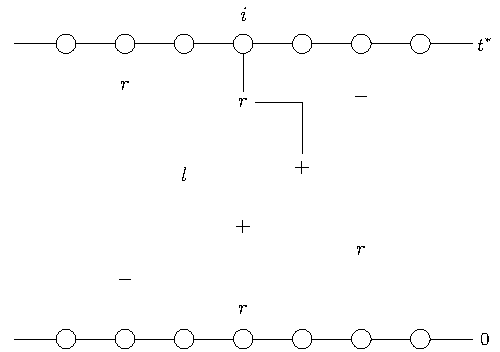
\includegraphics[width = 0.8\textwidth]{Figures/IsingCouplingTime/example_percolation_construction_rightleft.pdf}
		\caption[The update sequence for a section of the cycle and the corresponding update history from vertex i using the new update rules.]{The update sequence for a section of the cycle and the corresponding update history from vertex $i$ using the new update rules. Vertex $i$ takes the same spin as the spin it terminates at, in this case $+1$.}
		\label{fig:example percolation construction rightleft}
	\end{figure}

	We now see that as $t$ decreases from $t^*$, $\mathcal{H}_i(t)$ is a continuous-time random walk that dies at rate $\theta$, moves left at rate $(1 - \theta)/2$, and moves right at rate $(1 - \theta)/2$. The probability that $\mathcal{H}_i(0) \neq \emptyset$ is simply the probability that the continuous-time random walk survives until time $t = 0$. This immediately gives us the following probability which we will use repeatedly in what follows. Recalling \eqref{eq:prob equality of coupling and empty support},
	\begin{equation}
		\prob \left[ \mathscr{B}_{t^*}[i] \neq \mathscr{T}_{t^*}[i] \right] = 
		\prob \left[ \mathcal{H}_i(0) \neq \emptyset \right] = 
		\euler^{-\theta t^*}.
		\label{eq:1D bernoulli prob}
	\end{equation}
	since our histories die at rate $\theta$.

	\section{Problem Setup}
	In order to prove Theorem \ref{thm:Coupling Distribution on Cycle}, we will actually prove a stronger statement using Theorem \ref{thm: compound poisson approximation}. The general idea is that at some fixed time $t^*$ we will count the number of vertices at which the bottom and top chains differ. This number is a random variable, which we will call $W$, and we can bound the total variation distance of its distribution with that of an appropriate compound poisson distribution. As a special case, we can use this bound as a bound on the probability that $W$ is zero. Of course, if $W$ is zero then the top and bottom chains must have coupled and so we can use this to establish Theorem \ref{thm:Coupling Distribution on Cycle}.

	Bounding the total variation distance between $W$ and the compound Poisson will be done using compound Poisson approximation as described in \cite{Barbour2001-nh}. This paper reviews a number of different methods by which approximations may be made. The specific method that we will employ is based on Stein's method for the compound Poisson distribution, introduced in \cite{Barbour1992-mc}.

	We now make precise the ideas stated above.	Fix $z$ and a time of interest, $t_* = (z + \ln n)/\theta$. For each vertex $i \in G$, define indicators
	\begin{equation}
		X_i = 
		\begin{cases}
			1 & \mathscr{B}_{t^*}[i] \neq \mathscr{T}_{t^*}[i],\\
			0 & \mathscr{B}_{t^*}[i] = \mathscr{T}_{t^*}[i]
		\end{cases}
	\end{equation}
	and set $W = \sum_{i \in V} X_i$.
	Note that from \eqref{eq:1D bernoulli prob} we get
	\begin{equation}
		\label{eq:1D prob X_i}
		\prob[X_i = 1] = \euler^{-\theta t_*} = \frac{e^{-z}}{n}.
	\end{equation}
	% We create vertex sets
	% \begin{align}
	% 	B_i &= \{j\neq i : |j - i| \leq b_n \},\\
	% 	C_i &= \{j\notin B_i\cup \{i\}: |j - i| \leq c_n \},\\
	% 	D_i &= V \setminus (B_i \cup C_i \cup \{i\}).
	% \end{align}
	% where $b_n = \ln(n)$ and $c_n = \ln(n)^2$. 
	For each $i \in V$, decompose $W$ into $W = X_i + U_i + Z_i + W_i$ where
	\begin{align}
		U_i &= \sum_{j \in B_i} X_j, &
		Z_i &= \sum_{j \in C_i} X_j, &
		W_i &= \sum_{j \in D_i} X_j.
	\end{align}
	and $B_i, C_i$, and $D_i$ are the vertex sets
	\begin{align}
		B_i &= \{j\neq i : |j - i| \leq b_n \},\\
		C_i &= \{j\notin B_i\cup \{i\}: |j - i| \leq c_n \},\\
		D_i &= V \setminus (B_i \cup C_i \cup \{i\}).
	\end{align}
	We have some freedom in choosing $b_n$ and $c_n$; they are chosen to control the assymptotics of various quantities to be defined later. For this chapter, we will choose $b_n = \ln(n)$ and $c_n = \ln(n)^2$.

	We now define the quantities
	\begin{align}
		\lambda &= \sum_{i \in V} \expect\left[\frac{X_i}{X_i + U_i} \indicator[ X_i + U_i \geq 1] \right],\\
		\mu_l &= \frac{1}{l \lambda} \sum_{i \in V} \expect\left[ X_i \indicator[X_i + U_i = l] \right], && l\geq 1,
	\end{align}
	which will be the parameters of the approximating compound Poisson distribution to $W$. We also define
	\begin{align}
		\delta_1 &= \sum_{i \in V}  \sum_{k \geq 0} \prob[X_i = 1, U_i = k] \expect \left|\frac{\prob[X_i = 1, U_i = k|W_i]}{\prob[X_i = 1, U_i = k]} - 1 \right|,\\ 
		% \delta_2 &= \\
		% \delta_3 &= \\
		\delta_4 &= \sum_{i \in V} \left( \expect[X_i Z_i] + \expect[X_i] \expect[X_i + U_i + Z_i] \right),
	\end{align}
	% which we will require to vanish as $n \rightarrow \infty$.
	which we desire to be small for the compound Poisson approximation to be good.

	The following theorem (reworked from \cite{Barbour2001-nh}) bounds the distance between the distributions of $W$ and the approximating compound Poisson.

	\begin{theorem}[\cite{Barbour2001-nh}]
	\label{thm: compound poisson approximation}
		Let $W$, $\lambda$, $\vect{\mu}$, $\delta_1$ and $\delta_4$ be as defined above. Then
		\begin{equation}
			d_{\mathrm{TV}}(\mathscr{L}(W), \mathrm{CP}(\lambda, \vect{\mu})) \leq (\delta_1 + \delta_4)\euler^\lambda.
		\end{equation}
	\end{theorem}
	Note that $W$ is zero precisely when $T < t^*$ and so the events $\{W = 0\}$ and $\{T \leq t^*\}$ are the same. Furthermore, if $W'$ is compound Poisson with parameters $\lambda$ and $\vect{\mu}$ then $\prob[W' = 0] = \euler^{-\lambda}$. These observations lead to the following corollary of Theorem \ref{thm: compound poisson approximation}.
	\begin{corollary}
	\label{cor:bound distance prob[w=0] and e^-lambda}
	Let $T_n$ be the coupling time of the continuous-time heat-bath Glauber dynamics for the zero-field Ising model at inverse-temperature $\beta$ on the cycle $(\mathbb{Z}/n\mathbb{Z})$ and let $\delta_1$, $\delta_4$ and $\lambda$ be as defined above. Then
		\begin{equation}
			\left|\prob\left[T_n \leq \frac{z+\ln(n)}{\theta}\right] - \euler^{-\lambda}\right| \leq (\delta_1 + \delta_4)\euler^\lambda,
			\label{eq:bound distance prob[w=0] and e^-lambda}
		\end{equation}
		where $\theta = 1 - \tanh(2\beta)$.
	\end{corollary}	

	\section{Proof of Theorem \ref{thm:Coupling Distribution on Cycle}}
	\label{sec:proof thm coupling cycle}
	In this section we use Corollary \ref{cor:bound distance prob[w=0] and e^-lambda} to prove Theorem \ref{thm:Coupling Distribution on Cycle} by bounding $\lambda$ and showing that $\delta_1$ and $\delta_4$ go to zero as $n \rightarrow \infty$. This is done in Lemmas \ref{lem:1Dlambda}, \ref{lem:delta1 goes to 0}, and \ref{lem:delta4 goes to 0}. The proofs of these require some additional lemmas which have been deferred to Section \ref{sec:additional lemmas 1D}.

	We begin by bounding $\lambda$.
	\begin{lemma}
	\label{lem:1Dlambda}
		Using the above setup
		\begin{equation}
			\lim_{n \rightarrow \infty} \lambda = C_\theta \euler^{-z}
		\end{equation}
		where
		\begin{equation}
			\sqrt{\frac{\theta}{4 - 3\theta}} \leq C_\theta \leq 1.
		\end{equation}
	\end{lemma}
	NEED TO SHOW THAT THING ACTUALLY CONVERGES
	\begin{proof}
		\begin{align}
			\lambda &= \sum_{i \in V} \expect\left[\frac{X_i}{X_i + U_i} \indicator[ X_i + U_i \geq 1] \right]\\
				&= \sum_{i = 1}^n \prob(X_i = 1) \expect \left[\frac{1}{1 + U_i}| X_i = 1\right]\\
				&= \sum_{i = 1}^n \frac{\euler^{-z}}{n} \expect \left[\frac{1}{1 + U_i}| X_i = 1\right]\\
				&= \euler^{-z} \expect \left[\frac{1}{1 + U_i}| X_i = 1\right]
		\end{align}
		where we have used that $X_i$ is zero-one, \eqref{eq:1D prob X_i}, and the transitivity of the graph.
		Clearly 
		\begin{align}
			\expect \left[\frac{1}{1 + U_i}| X_i = 1\right] \leq 1
		\end{align}
		and so $C_\theta \leq 1$.

		By Jensen's inequality
		\begin{align}
			\expect \left[\frac{1}{1 + U_i}| X_i = 1\right] &\geq \frac{1}{\expect[1 + U_i | X_i = 1]}\\
				&= \frac{1}{1 + \expect[U_i | X_i = 1]}.
		\end{align}
		so in order to find a lower bound for $\lambda$ we will find an upper bound to $\expect[U_i | X_i = 1]$. Now
		\begin{align}
			\expect[U_i | X_i = 1] &= \sum_{j \in B_i} \prob[X_j = 1| X_i = 1]\\
				&= \sum_{k=1}^{b_n} \sum_{|j - i| = k} \prob[X_j = 1| X_i = 1]\\
				&= 2 \sum_{k=1}^{b_n} \prob[X_{i+k} = 1 | X_i = 1]
		\end{align}
		where we have used the symmetry of $X_{i+k}$ and $X_{i -k}$ in the last step. From Lemma \ref{lem:X_i+k given X_i}, 
		\begin{align}
			\expect[U_i | X_i = 1] &\leq 2 \sum_{k = 1}^{b_n} \left(\frac{e^{-z}}{n} + 2 \left(\frac{2 - \sqrt{\theta(4 - \theta)}}{2 - \theta}\right)^k\right)\\
				&< 2 \sum_{k = 1}^{b_n} \frac{e^{-z}}{n} + 4\sum_{k = 1}^\infty \left(\frac{2 - \sqrt{\theta(4 - \theta)}}{2 - \theta}\right)^k\\
				&= \frac{2 b_n}{n}e^{-z} + 2\left(\sqrt{\frac{4}{\theta} - 1} - 1\right).
		\end{align}
		Finally, as $n \rightarrow \infty$ the first term vanishes and
		\begin{align}
			\lim_{n \rightarrow \infty} \lambda \geq \frac{e^{-z}}{2\sqrt{\frac{4}{\theta} - 1} - 1}.
		\end{align}
	\end{proof}

	Blahblahblah, any remarks about $\lambda$ go here.

	\begin{lemma}
	\label{lem:delta1 goes to 0}
		\begin{equation}
			\lim_{n\rightarrow\infty} \delta_1 = 0
		\end{equation}
	\end{lemma}
	\begin{proof}
		\begin{align}
			\delta_1 &= \sum_{i = 1}^n \sum_{k = 0}^{2 b_n} \prob[X_i = 1, U_i = k] \expect \left| \frac{\prob[X_i = 1, U_i = k|W_i]}{\prob[X_i = 1, U_i = k]} - 1 \right|\\
			&= n \sum_{k = 0}^{2 b_n} \expect \left|\prob[X_i = 1, U_i = k|W_i] - \prob[X_i = 1, U_i = k] \right|%\\
			\label{eq: delta1 line 2}
			% &\leq n \sup_{W_i} \sum_{k = 0}^{2 b_n} \left| \prob[X_i = 1, U_i = k|W_i] - \prob[X_i = 1, U_i = k] \right|
		\end{align}
		Let $A$ be the event that the history of a vertex in $D_i$ merges with the history of a vertex in $B_i \cup \{i\}$. More formally,
		\begin{equation}
			A = \{ \exists j \in B_i \cup \{i\}, l \in D_i : \mathcal{H}_j \cap \mathcal{H}_l \neq \emptyset\}.
		\end{equation}
		We note that if $A$ does not happen, then $W_i$ cannot affect $X_i$ or $U_i$. That is,
		\begin{equation}
			\prob[X_i = 1, U_i = j | A^\complement, W_i] = \prob[X_i = 1, U_i = j | A^\complement].
		\end{equation} 
		Continuing on from \eqref{eq: delta1 line 2}, we split the probabilities into
		\begin{align}
			\delta_1 &= n \sum_{k = 0}^{2 b_n} \expect \left| \prob[X_i = 1, U_i = k|W_i, A]\prob[A|W_i] - \prob[X_i = 1, U_i = k| A]\prob[A] + \vphantom{A^\complement} \right.\\
			&\hphantom{= .} \left.\prob(X_i = 1, U_i = k | A^\complement) (\prob[A^\complement|W_i] - \prob[A^\complement]) \right| \notag \\
			&\leq n (2b_n+1) \expect\left[ \prob[A|W_i] + \prob[A] + \left|\prob[A^\complement|W_i] - \prob[A^\complement]\right|\right]\\
			&= n (2b_n + 1) \expect\left[ \prob[A|W_i] + \prob[A] + \left|1 - \prob[A|W_i] - (1 - \prob[A])\right|\right]\\
			&\leq n (2b_n + 1) \expect\left[ \prob[A|W_i] + \prob[A] + \prob[A|W_i] + \prob[A])\right]\\
			&= 2 n (2b_n + 1) \left(\expect[\prob[A|W_i]] + \prob[A]\right)\\
			&= 4 n (2b_n + 1) \prob[A]
		\end{align}

		Let $A_{j,k}$ denote the event that the histories of vertices $j$ and $k$ merge. That is,
		\begin{equation}
			A_{j,k} = \{\mathcal{H}_j \cap \mathcal{H}_k \neq \emptyset\}.
		\end{equation}
		By a union bound,
		\begin{align}
			\delta_1 &\leq 4 n (2b_n + 1) \sum_{j \in B_i \cup \{i\}} \sum_{k \in D_i} \prob[A_{j,k}]\\
			&\leq 8n^2(2b_n + 1)^2  \left(\frac{1 - \sqrt{\theta(2 - \theta)}}{1 - \theta}\right)^{c_n - b_n}
		\end{align}
		by Lemma \ref{lem: A_ij bound}. This goes to $0$ as $n \rightarrow \infty$.
	\end{proof}

	\begin{lemma}
	\label{lem:delta4 goes to 0}
		\begin{equation}
			\lim_{n\rightarrow\infty} \delta_4 = 0
		\end{equation}
	\end{lemma}
	\begin{proof}
		\begin{align}
			\delta_4 &= \sum_{i = 1}^n \left(\expect[X_i Z_i] + \expect[X_i]\expect[X_i + U_i + Z_i]\right)\\
				&= \sum_{i=1}^n \expect[X_i Z_i] + \euler^{-z} \sum_{j \in \{i\}\cup B_i \cup C_i} \expect[X_j]\\
				&= n \expect[X_i Z_i] + \frac{2\euler^{-2z}c_n}{n}\\
				&= n \prob[X_i = 1] \expect[Z_i | X_i = 1] + \frac{2\euler^{-2z}c_n}{n}\\
				&= \euler^{-z}\expect[Z_i | X_i = 1] + \frac{2\euler^{-2z}c_n}{n}
		\end{align}
		Now
		\begin{align}
			\expect[Z_i | X_i = 1] &= \sum_{j \in C_i} \prob[X_j = 1 | X_i = 1]\\
			&= 2 \sum_{k = b_n + 1}^{c_n} \prob[X_{i+k} = 1 | X_i = 1]
		\end{align}
		From Lemma \ref{lem:X_i+k given X_i},
		\begin{align}
			\expect[Z_i | X_i = 1] &\leq 2 \sum_{k = b_n + 1}^{c_n} \left(\frac{e^{-z}}{n} + 2\left(\frac{2 - \sqrt{\theta(4 - \theta)}}{2 - \theta}\right)^k\right)\\
				&\leq \frac{2(c_n - b_n)\euler^{-z}}{n} + 4(c_n - b_n)\left(\frac{2 - \sqrt{\theta(4 - \theta)}}{2 - \theta}\right)^{b_n + 1}.
		\end{align}
		Altogether
		\begin{equation}
			\delta_4 \leq \frac{2(c_n - b_n)\euler^{-z}}{n} + 4(c_n - b_n)\left(\frac{2 - \sqrt{\theta(4 - \theta)}}{2 - \theta}\right)^{b_n + 1} + \frac{2\euler^{-2z}c_n}{n}
		\end{equation}
		which goes to $0$ as $n \rightarrow \infty$.
	\end{proof}

	\section{Additional Lemmas}
	\label{sec:additional lemmas 1D}
	\begin{lemma}
		\label{lem: A_ij bound}
		Let $A_{i,j}$ be the event that the update history of vertex $i$ merges with the update history of vertex $j$. Then
		\begin{equation}
			\prob[A_{i,j}] \leq 2\left(\frac{1 - \sqrt{\theta(2 - \theta)}}{1 - \theta}\right)^k
		\end{equation}
		where $k = |i - j|$.
	\end{lemma}
	\begin{proof}
		We note that, while the update histories survive, the distance between the update histories of $i$ and $j$ is a birth and death process that starts at $k = |i - j|$ and has birth and death rates, $\lambda = \mu = 1 - \theta$. Let $P(t)$ be such a process and define $s_0  = \inf\{t : P(t) = 0\}$ to be the first time the process reaches zero (this corresponds to the update histories merging). Let $s_d$ be exponentially distributed with rate $2\theta$ (this corresponds to the first time that one of the update histories dies). Then
		\begin{align}
		 	\prob[A_{i,j}] \leq 2 \prob_k(s_0 < s_d)
		 \end{align} 
		 where $\prob_k$ indicates that $P(0) = k$. The factor of two comes from the fact that the update histories may meet by going the other direction around the cycle.

		 At any time before $s_d$ there are three possibilities for what can happen to $P$ next. Either the next event is a birth with probability $(1 - \theta)/2$, the next event is a death with the same probability or we reach time $s_d$ with probability $\theta$. Writing $\zeta_k = \prob_k(s_0 < s_d)$ this gives us the recurrence relation
		 \begin{align}
		 	\zeta_k = \frac{1 - \theta}{2} \zeta_{k-1} + \frac{1 - \theta}{2} \zeta_{k+1}
		 \end{align}
		 which is subject to the conditions 
		 \begin{align}
		 	\label{eq:zetacondition1}
		 	\zeta_0 &= 1\\
		 	\zeta_k &\leq 1, \, \forall k \in \mathbb{N}.
		 	\label{eq:zetacondition2}
		 \end{align} 
		 This recurrence has characteristic equation
		 \begin{align}
		 	x^2 - \frac{2}{1 - \theta} x + 1 = 0
		 \end{align}
		 which has roots
		 \begin{align}
		 	r_1 &= \frac{1 + \sqrt{\theta(2 - \theta)}}{1 - \theta}\\
		 	r_2 &= \frac{1 - \sqrt{\theta(2 - \theta)}}{1 - \theta}
		 \end{align}
		 and so
		 \begin{align}
		 	\zeta_k = a r_1^k + b r_2^k
		 \end{align}
		 where $a$ and $b$ are constants to be determined from \eqref{eq:zetacondition1} and \eqref{eq:zetacondition2}. We note that $r_1 \geq 1, \forall \theta \in [0,1]$ and so from \eqref{eq:zetacondition2} we have that $a = 0$. Finally from \eqref{eq:zetacondition1}, $b = 1$ and so
		 \begin{equation}
		 	\zeta_k = \left(\frac{1 - \sqrt{\theta(2 - \theta)}}{1 - \theta}\right)^k.
		 \end{equation}
	\end{proof}

	\begin{lemma}
	\label{lem:A_ij bound conditioned}
		Let $A_{i,j}$ be the event that the update history of vertex $i$ merges with the update history of vertex $j$. Then
		\begin{equation}
			\prob[A_{i,j}|X_{j} = 1] \leq 2\left(\frac{2 - \sqrt{\theta(4 - \theta)}}{2 - \theta}\right)^k.
		\end{equation}
		where $k = |i - j|$.
	\end{lemma}
	\begin{proof}
		We first must deal with the effect that conditioning on $X_j = 1$ has on the probability that the two update histories merge. For the history of vertex $j$ to survive, all updates along the history must be non-oblivious updates. We also note that conditioning on the history of vertex $j$ surviving should not result in an increase in the overall rate of updates (since each update is a chance that the history will die). By this reasoning, 
		\begin{equation}
			\prob[\mathcal{H}_i \cap \mathcal{H}_j \neq \emptyset | X_j = 1] \leq \prob[\mathcal{H}_i \cap \bar{\mathcal{H}}_j]
		\end{equation}
		where $\bar{\mathcal{H}}_j$ is an undying random walk that starts at $j$ and going backwards in time from $t^*$ moves right at rate 1/2 and left at rate 1/2.

		We note that, while $\mathcal{H}_i$ survives, the distance between $\mathcal{H}_i$ and $\bar{\mathcal{H}}_j$ is a birth and death process that starts at $k = |i - j|$ and has birth and death rates, $\lambda = \mu = (2 - \theta)/2$. Let $P(t)$ be such a process and define $s_0  = \inf\{t : P(t) = 0\}$ to be the first time the process reaches zero (this corresponds to the update histories merging). Let $s_d$ be exponentially distributed with rate $\theta$ (this corresponds to the update history of vertex $i$ dying). Then
		\begin{align}
		 	\prob[A_{i,j} | X_j = 1] \leq \prob[\mathcal{H}_i \cap \bar{\mathcal{H}}_j] \leq 2 \prob_k(s_0 < s_d)
		 \end{align} 
		 where $\prob_k$ indicates that $P(0) = k$. The factor of two comes from the fact that the update histories may meet by going in either direction around the cycle.

		 At any time before $s_d$ there are three possibilities for what can happen to $P$ next. Either the next event is a birth with probability $(2 - \theta)/4$, the next event is a death with the same probability or we reach time $s_d$ with probability $\theta/2$. Writing $\zeta_k = \prob_k(s_0 < s_d)$ this gives us the recurrence relation
		 \begin{align}
		 	\zeta_k = \frac{2 - \theta}{4} \zeta_{k-1} + \frac{2 - \theta}{4} \zeta_{k+1}
		 \end{align}
		 which is subject to the conditions 
		 \begin{align}
		 	\label{eq:zetacondition1_cond}
		 	\zeta_0 &= 1\\
		 	\zeta_k &\leq 1, \, \forall k \in \mathbb{N}.
		 	\label{eq:zetacondition2_cond}
		 \end{align} 
		 This recurrence has characteristic equation
		 \begin{align}
		 	x^2 - \frac{4}{2 - \theta} x + 1 = 0
		 \end{align}
		 which has roots
		 \begin{align}
		 	r_1 &= \frac{2 + \sqrt{\theta(4 - \theta)}}{2 - \theta}\\
		 	r_2 &= \frac{2 - \sqrt{\theta(4 - \theta)}}{2 - \theta}
		 \end{align}
		 and so
		 \begin{align}
		 	\zeta_k = a r_1^k + b r_2^k
		 \end{align}
		 where $a$ and $b$ are constants to be determined from \eqref{eq:zetacondition1_cond} and \eqref{eq:zetacondition2_cond}. We note that $r_1 \geq 1, \forall \theta \in [0,1]$ and so from \eqref{eq:zetacondition2_cond} we have that $a = 0$. Finally from \eqref{eq:zetacondition1_cond}, $b = 1$ and so
		 \begin{equation}
		 	\zeta_k = \left(\frac{2 - \sqrt{\theta(4 - \theta)}}{2 - \theta}\right)^k.
		 \end{equation}
	\end{proof}

	\begin{lemma}
		\label{lem:X_i+k given X_i}
		\begin{equation}
			\label{eq:prob X_i+k = 1|X_i = 1}
			\prob[X_{i+k} = 1| X_i = 1] \leq \frac{e^{-z}}{n} + 2\left(\frac{2 - \sqrt{\theta(4 - \theta)}}{2 - \theta}\right)^k.
		\end{equation}
	\end{lemma}
	\begin{proof}
		There are two ways in which the update history of vertex $i+k$ can survive until time $0$. The update history can survive without intersecting with the update history of vertex $i$ or the update history of vertex $i+k$ can survive long enough to merge with the update history of vertex $i$ (whose surival we are conditioning on). (Note that these events are not mutually exclusive as the update history of vertex $i+k$ could merge with the update history of vertex $i$ after it reaches time $0$.) So we have
		\begin{align}
			\prob[X_{i+k} = 1| X_i = 1] &\leq \prob[X_{i+k} = 1] + \prob[A_{i,i+k} | X_i = 1].
		\end{align}
		The result follows from \eqref{eq:1D prob X_i} and Lemma \ref{lem:A_ij bound conditioned}.
	\end{proof}